% Modle pour rapport de Travail de Fin d'Etudes de l'Ecole Centrale de Lyon
% version 0.1
% 2009-07-24
% par Steren Giannini (steren.giannini@gmail.com)
% Ce modèle est mis  disposition selon le Contrat "Creative Commons Paternité-Partage des Conditions Initiales  l'Identique 3.0 Unported"
% http://creativecommons.org/licenses/by/3.0/

\documentclass[12pt,a4paper]{article}
%Chargement des packages
\usepackage[utf8]{inputenc} % l'encodage des fichiers est utf-8, mettre [latin1] si necessaire
\usepackage[french]{babel} %le rapport est en français 
\usepackage{amsmath}
\usepackage{amsfonts}
\usepackage{amssymb}
\usepackage{graphicx} %pour afficher des images
\usepackage{float}	%pour forcer le placement des images.
\usepackage{geometry} %pour la modification des marges
\usepackage{fancyhdr} %pour modification des pieds de page
\usepackage{longtable}
\usepackage{listings}
\usepackage{subfigure}
\usepackage{hyperref} %pour que les références soient des liens hypertextes
\usepackage[usenames,dvipsnames]{color} % pour les textes en gris


% Comment utiliser : 
% - la page de titre est à personnaliser (title/title.tex)
% - le contenu est à rédiger dans le répertoire pages/, s'inspirer des exemples présents dans ce modèle.
% - les annexes sont à rédiger dans le répertoire appendix/
% - la bibliographie utilise BibTex (fichier biblio.bib)
% - les variables suivantes sont à remplir :
\newcommand{\TitreRapport}{Titre du TFE}
\newcommand{\DateRapport}{2009}
\newcommand{\AuteurRapport}{Prénom Nom}
\newcommand{\NomEntreprise}{Nom Entreprise}

%définition des marges
\geometry{hmargin=2.5cm, vmargin=2.5cm } 

%utilisation des puces anglaises.
%attention, il faut avoir une version récente de frenchb.ldf. 
\frenchbsetup{StandardItemLabels}

%Définition des en-têtes et pieds de page
\renewcommand{\headrulewidth}{0pt}
\renewcommand{\footrulewidth}{0pt}
\fancyhead[C]{ \textcolor{Gray}{\small\TitreRapport}}
\fancyfoot[C]{ \textcolor{Gray}{ \small\AuteurRapport ~~ \vline ~~ TFE ~~ \vline ~~ \DateRapport }}

\fancyfoot[LE, RO]{\thepage}
\fancyfoot[RE, LO]{
\includegraphics[width=1.8cm]{style/images/logo_small.png}}

\fancyhead[L,R]{}


% définition du tire, de la date et de l'auteur du document
\title{\TitreRapport}
\date{\DateRapport}
\author{\AuteurRapport}

\makeatletter

\renewcommand\maketitle{
  \begin{titlepage}
  
  	\begin{center}
    	
\includegraphics[height=2.3cm]{title/images/logo_centrale.png}
    	\hspace{\stretch{1}}
    	
\includegraphics[height=2.3cm]{title/images/logo_entreprise.png}
    
    \vspace{\stretch{0.5}}
    	
		  \begin{tabular*}{1.0\textwidth}{l @{\extracolsep{\fill}} r}
					École Centrale de Lyon 				& \NomEntreprise 				\\
					TFE \@date 							& Ville du lieu du Stage 		\\
			\end{tabular*}

  	\vspace{\stretch{1.5}}
  	
 		{\large \bf \textsf{Rapport Final de Travail de Fin d'études} \\}
    \vspace{0.5cm}
    {\LARGE \bf \textsf{\@title}\\}
    \vspace{0.5cm}
    {\large \it \textsf{\@author}\\}
  
	  \vspace{\stretch{2}}
	  
\includegraphics[width=1.0\textwidth]{title/images/logo_illustration.png}
	  \vspace{\stretch{2}}
	    
		  \begin{tabular*}{1.0\textwidth}{|l @{\extracolsep{\fill}} r|}
				\hline
					Tuteurs : 						& Option : (sigle développé) 	\\
					&\\
					\textit{ECL} :				& 														\\
					Nom, Prénom Tuteur 1 	& Filière : (sigle développé)	\\
					Nom, Prénom Tuteur 2 	& 														\\
					&\\
					\textit{Entreprise} :	& 														\\		
					Nom, Prénom Tuteur 1	& Métier : (sigle développé)		\\
					Nom, Prénom Tuteur 2	& 														\\	
				\hline
			\end{tabular*}
		\end{center}\par
    
  \end{titlepage}
  \setcounter{footnote}{0}
  
%  \global\let\thanks\relax
%  \global\let\maketitle\relax
%  \global\let\@thanks\@empty
%  \global\let\@author\@empty
%  \global\let\@date\@empty
%  \global\let\@title\@empty
%  \global\let\title\relax
%  \global\let\author\relax
%  \global\let\date\relax
%  \global\let\and\relax
}


\makeatother


\begin{document}
\pagestyle{fancy}

\maketitle
		\newpage
\section*{Remerciements}
Insérez ici vos remerciements.

		\newpage
\section*{Résumé du rapport :}
Insérez ici le résumé en français

\subsubsection*{Mots-clés libres :}
Insérez ici les mots clés en français (séparés par des points-virgules)

		\newpage
\section*{Abstract:}
Insérez ici le résumé en anglais

\subsubsection*{Keywords:}
Insérez ici les mots clés en anglais (séparés par des points-virgules)

		\newpage
\tableofcontents
        \newpage
\listoffigures
\listoftables
		\newpage
\section*{Introduction}
\addcontentsline{toc}{section}{Introduction}
Insérez ici votre introduction.

        \newpage
\section{Titre1}

Non ergo erunt homines deliciis diffluentes audiendi, si quando de amicitia, quam nec usu nec ratione habent cognitam, disputabunt \footnote{Exemple de note de bas de page}.

\subsection{Titre de niveau 2}

Isdem diebus Apollinaris Domitiani gener, paulo ante agens palatii Caesaris curam, ad Mesopotamiam missus a socero per [...].

\subsubsection{Titre de niveau 3}
Isdem diebus Apollinaris Domitiani gener, paulo ante agens palatii Caesaris curam, ad Mesopotamiam missus a socero per militares numeros immodice scrutabatur, an quaedam altiora meditantis iam Galli secreta susceperint scripta, qui conpertis Antiochiae gestis per minorem Armeniam lapsus Constantinopolim petit exindeque per protectores retractus artissime tenebatur.

\begin{itemize}
\item Liste a puces 1
			\begin{itemize}
			\item Liste a puces 2
						\begin{itemize}
						\item Liste a puces 3
						\end{itemize}
			\end{itemize}
\end{itemize} 

\paragraph{Titre de niveau 4}
Non ergo erunt homines deliciis diffluentes audiendi, si quando de amicitia, quam nec usu nec ratione habent cognitam, disputabunt.

\begin{figure}[H]
	\center
	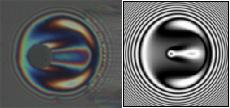
\includegraphics[width=0.4\textwidth]{body/images/figure_example.png} 
	\caption{Exemple de figure avec légende}
	\label{fig:exemple}
\end{figure}

\subparagraph{Titre de niveau 5}

Isdem diebus Apollinaris Domitiani gener, paulo ante agens palatii Caesaris curam, ad Mesopotamiam missus a socero per militares numeros immodice scrutabatur, an quaedam altiora meditantis iam Galli secreta susceperint scripta, qui conpertis Antiochiae gestis per minorem Armeniam lapsus Constantinopolim petit exindeque per protectores retractus artissime tenebatur.

Titre de niveau 6
Non ergo erunt homines deliciis diffluentes audiendi,


\subsection{Titre de niveau 2}

Isdem diebus Apollinaris Domitiani gener, paulo ante agens palatii Caesaris curam, ad Mesopotamiam missus a socero per [...].


        \newpage
\section{Titre2}

Non ergo erunt homines deliciis diffluentes audiendi, si quando de amicitia, quam nec usu nec ratione habent cognitam, disputabunt.

Exemple de citation \cite{sheffer2006mpm}

		\newpage
\section*{Conclusion}
\addcontentsline{toc}{section}{Conclusion}
Insérez ici votre conclusion.

		\newpage
\bibliographystyle{unsrt}
\bibliography{biblio} 
		\newpage
\appendix
\section{Titre de votre première annexe}

Insérez ici votre premier document d’annexe.


\end{document}
